\documentclass[10pt,a4paper]{article}
\usepackage[utf8]{inputenc}
\usepackage[T1]{fontenc}
\usepackage[brazil]{babel}
\usepackage[margin=1.7cm]{geometry}
\usepackage{booktabs}
\usepackage{enumitem}
\usepackage{microtype}
\usepackage{graphicx}
\usepackage{xcolor}
\usepackage{tikz}
\newcommand{\tikzmark}[1]{\tikz[overlay,remember picture,baseline=0pt]\node[inner sep=0pt,outer sep=0pt] (#1) at (0,0) {};}
\usepackage[font=small,labelfont=bf]{caption}

\setlength{\parindent}{0pt}
\setlength{\parskip}{3pt}
\setlist{nosep,leftmargin=1.2em}
\pagestyle{empty}

\title{\vspace{-1.4cm}\textbf{Relat\'orio: An\'alise XAI do Impacto da IA nas Profiss\~oes (2030)}\\[2pt]
\normalsize \'Etica em Intelig\^encia Artificial --- Explicabilidade com LIME e SHAP\vspace{-0.4cm}}
\author{\small Jefferson Cunha --- \texttt{jefferson.cunha@ufpe.br}\\[1pt]
\small Disciplina: \'Etica e Intelig\^encia Artificial --- 2\textsuperscript{o} sem/2026 --- Prof.\ Geber Ramalho}
\date{\vspace{-0.6cm}}


\begin{document}
\maketitle

\textbf{Metodologia.} Usei o \textit{dataset} \textit{AI Impact on Jobs 2030} (3000 registros, 20 cargos, 10 \textit{skills}). O alvo \'e \texttt{Automation\_}\allowbreak\texttt{Probability\_}\allowbreak\texttt{2030}. Treinei um \texttt{RandomForestRegressor} (\texttt{random\_state}=101, 70/30) e expliquei com SHAP (\texttt{TreeExplainer}, 500 inst\^ancias) e LIME (inst\^ancia 221, \texttt{seed}=42). \texttt{Education\_Level} \'e ordinal e \texttt{Job\_Title} \'e \textit{one-hot}. \texttt{Risk\_Category} foi removida por \textbf{vazamento do alvo} (Low 0,05--0,30; Medium 0,31--0,70; High 0,71--0,95). Experimentos: \textbf{Exp1} remove \texttt{Skill\_1} e \texttt{Skill\_5} (maiores $|$corr$|$ com o alvo entre as \textit{skills}: $+0{,}031$ e $-0{,}026$); \textbf{Exp2} remove \texttt{AI\_Exposure\_Index} e \texttt{Years\_Experience} (corr.\ $+0{,}014$ e $-0{,}018$).

\section*{1. Desempenho preditivo}
\begin{center}\small
\begin{tabular}{@{}lccccc@{}}
\toprule
Modelo & R$^2$ & RMSE & MAE & R$^2$ (5 \textit{seeds}) & Predi\c{c}\~ao inst.\ 221 \\ \midrule
Baseline & 0,8494 & 0,0983 & 0,0819 & 0,8485 $\pm$ 0,0013 & 0,146 \\
Exp1 (sem \texttt{Skill\_1}, \texttt{Skill\_5}) & 0,8498 & 0,0982 & 0,0815 & 0,8488 $\pm$ 0,0010 & 0,149 \\
Exp2 (sem \texttt{AI\_Exp.}, \texttt{Years\_Exp.}) & 0,8482 & 0,0987 & 0,0825 & 0,8475 $\pm$ 0,0014 & 0,145 \\ \bottomrule
\end{tabular}
\end{center}
Valor real da inst\^ancia 221: 0,23. As tr\^es vers\~oes diferem em $\le$0,002 de R$^2$, o que \'e da ordem do desvio entre \textit{seeds} do Random Forest. Ou seja, \textbf{remover essas quatro vari\'aveis n\~ao altera o modelo de forma mensur\'avel}.

\section*{2. SHAP --- interpreta\c{c}\~ao global}
\begin{figure}[h]\centering
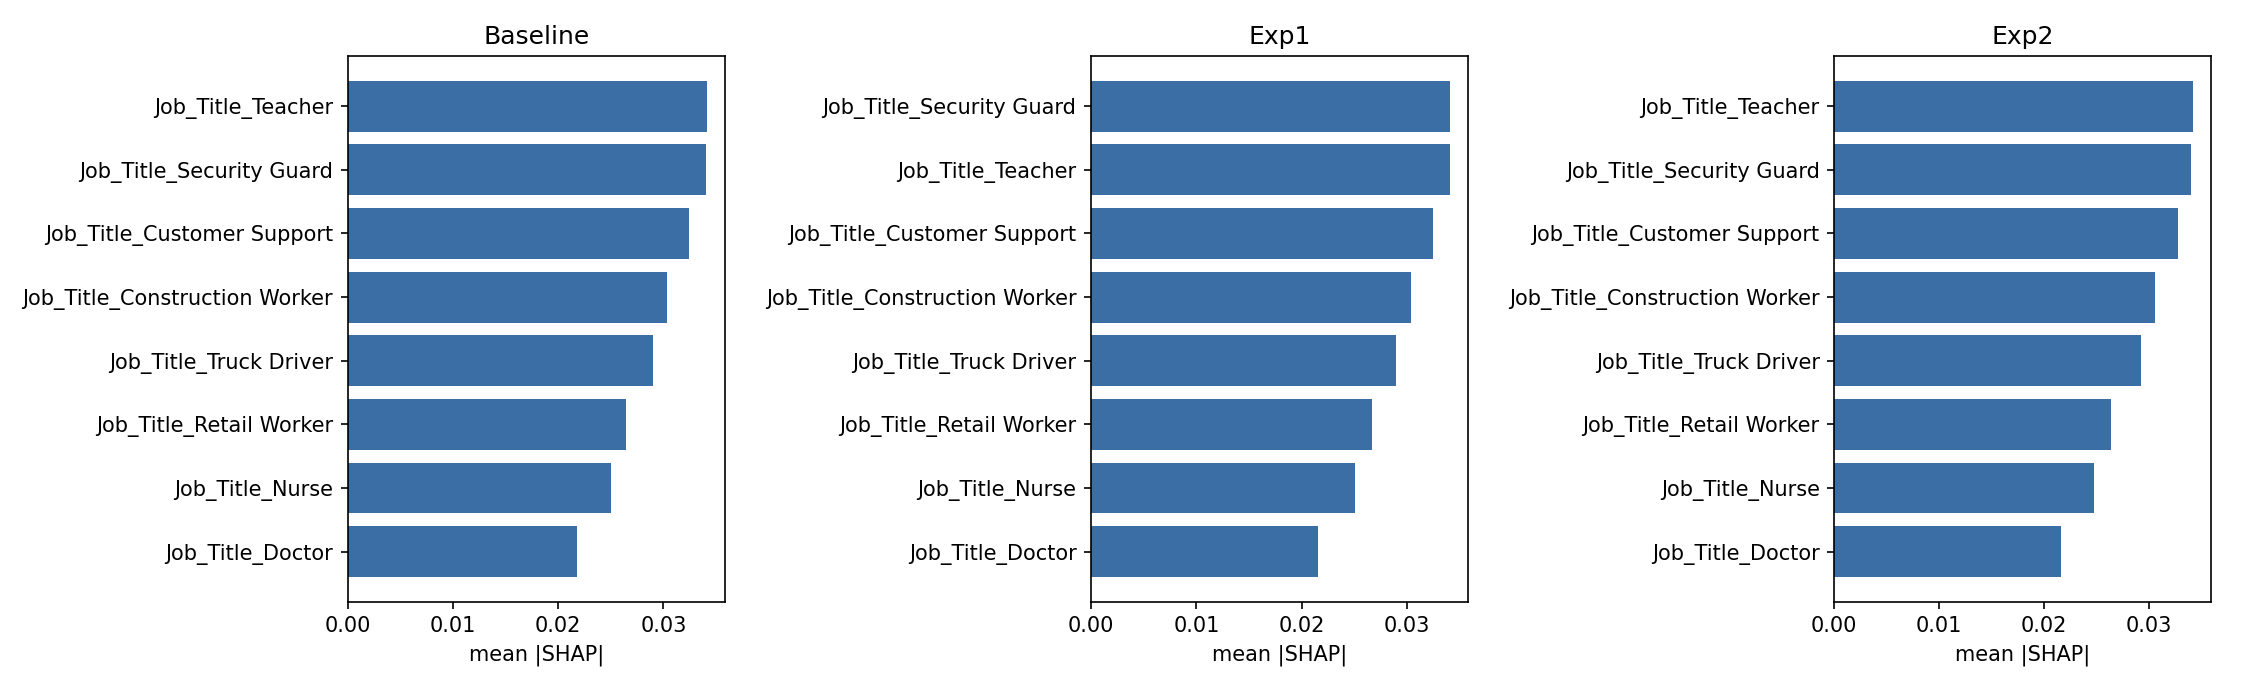
\includegraphics[width=\linewidth]{figs/shap_global.png}
\caption{Import\^ancia global (m\'edia de $|$SHAP$|$, 8 maiores) nas tr\^es vers\~oes.}
\end{figure}
As colunas \texttt{Job\_Title\_*} somam \textbf{0,271 dos 0,307} de import\^ancia total no baseline (\textbf{88\%}). As dez maiores s\~ao todas de cargo (\texttt{Teacher} 0,034; \texttt{Security Guard} 0,034; \texttt{Customer Support} 0,032). As dez \textit{skills} juntas somam apenas 0,022 (7\%), e as demais vari\'aveis (sal\'ario, experi\^encia, escolaridade, exposi\c{c}\~ao \`a IA, crescimento tecnol\'ogico) completam o resto, abaixo de 0,04. Nos Exp1 e Exp2 a import\^ancia dos cargos muda no quarto decimal (0,2713 e 0,2722): o ranking \'e id\^entico.

\section*{3. LIME --- interpreta\c{c}\~ao local}
\begin{figure}[h]\centering
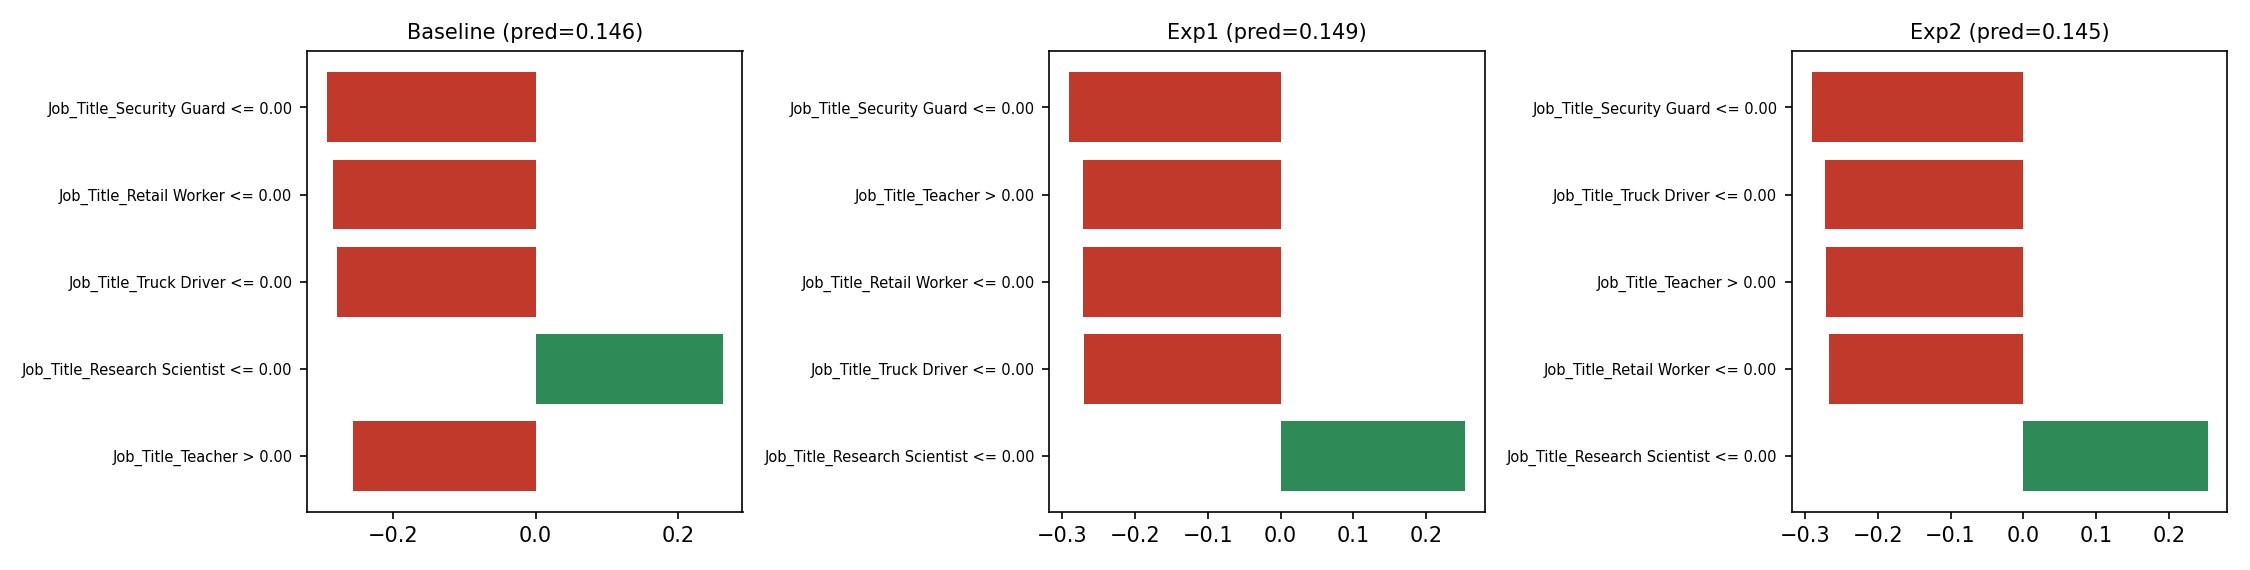
\includegraphics[width=\linewidth]{figs/lime_inst.png}
\caption{LIME da inst\^ancia 221 (5 \textit{features}), vermelho reduz e verde aumenta a probabilidade.}
\end{figure}
Nas tr\^es vers\~oes as cinco \textit{features} s\~ao \texttt{Job\_Title\_*}, com pesos de $\pm$0,25 a 0,29 (por ex., \texttt{Security Guard} $\le 0$: $-0{,}29$; \texttt{Research Scientist} $\le 0$: $+0{,}25$). Isto \'e coerente com o SHAP: a predi\c{c}\~ao baixa (0,15) vem de o cargo da pessoa n\~ao ser um dos de alto risco. Repetindo o LIME com 20 \textit{seeds}, \textbf{100\%} das \textit{features} do top-5 foram cargos nos tr\^es modelos, mas houve 9 conjuntos distintos de top-5. A ordem e quais cargos aparecem variam por amostragem do LIME, ent\~ao diferen\c{c}as entre execu\c{c}\~oes n\~ao devem ser lidas como efeito dos experimentos.

\section*{4. Discuss\~ao e melhor modelo}
\begin{itemize}
  \item \textbf{O modelo \'e praticamente uma tabela por cargo.} Com 88\% da import\^ancia em \texttt{Job\_Title}, as demais correla\c{c}\~oes ($|r|\le 0{,}03$ com o alvo) s\~ao ru\'ido. As explica\c{c}\~oes de SHAP e LIME concordam em subst\^ancia, o que d\'a confian\c{c}a \`a interpreta\c{c}\~ao e indica que o \textit{dataset} \'e provavelmente sint\'etico.
  \item \textbf{Melhor modelo.} O Exp1 tem o melhor desempenho num\'erico (R$^2$ 0,8498), mas a vantagem de 0,0004 \'e menor que o desvio entre \textit{seeds}. Recomendo o \textbf{Exp1}: desempenho equivalente ou ligeiramente melhor, duas \textit{features} a menos e explica\c{c}\~oes id\^enticas. O Exp2 \'e o pior numericamente, ainda que dentro do ru\'ido.
  \item \textbf{Sem rela\c{c}\~ao causal.} N\~ao se pode concluir que \textit{skills}, experi\^encia ou exposi\c{c}\~ao \`a IA n\~ao afetam a automa\c{c}\~ao real. Apenas que, neste \textit{dataset}, n\~ao carregam sinal.
\end{itemize}

\section*{5. Reflex\~oes \'eticas e limita\c{c}\~oes}
\begin{itemize}
  \item \textbf{Julgar pessoas pelo cargo.} Um modelo que decide pelo cargo trata indiv\'iduos como m\'edia da categoria: um(a) professor(a) altamente qualificado(a) recebe o mesmo risco que qualquer outro. Para pol\'iticas de requalifica\c{c}\~ao, isso \'e um \textit{proxy} grosseiro e pode estigmatizar profiss\~oes. XAI \'e o que torna essa depend\^encia vis\'ivel.
  \item \textbf{Vazamento.} Sem remover \texttt{Risk\_Category}, o modelo apenas reconstruiria o alvo e SHAP/LIME explicariam um artefato. Explicabilidade s\'o \'e confi\'avel se o modelo o for.
  \item \textbf{Escopo.} O enunciado fala em programa\c{c}\~ao, mas usei todos os cargos do \textit{dataset}, sem filtro. O LIME trata \textit{one-hot} como cont\'inuo (\texttt{<= 0,00}); declarar \texttt{categorical\_features} tornaria o texto mais leg\'ivel.
\end{itemize}

\section*{6. \textit{Lessons learned}}
A explicabilidade revelou o que as m\'etricas escondiam: um R$^2$ de 0,85 vindo quase inteiramente de uma \'unica vari\'avel categ\'orica. Remover \textit{features} sem sinal n\~ao mudou desempenho nem explica\c{c}\~ao, e o LIME precisa ser repetido com \textit{seeds} diferentes antes de se interpretar uma inst\^ancia isolada.

\end{document}
